	%%%%%%%%%%%%%%%%%%%%%%%%%%%%%%%%%%%%%%%%%%%%%%%%%%%%%%%%%%%%%%%%
%
%  Template for homework of Introduction to Machine Learning.
%
%  Fill in your name, lecture number, lecture date and body
%  of homework as indicated below.
%         
%%%%%%%%%%%%%%%%%%%%%%%%%%%%%%%%%%%%%%%%%%%%%%%%%%%%%%%%%%%%%%%%
\documentclass[11pt,letter,notitlepage]{article}
%Mise en page
\usepackage[left=2cm, right=2cm, lines=45, top=0.8in, bottom=0.7in]{geometry}
\usepackage{fancyhdr}
\usepackage{fancybox}
\usepackage{graphicx}
\usepackage{pdfpages}
\usepackage{enumitem}
\usepackage{algorithm}
\usepackage{algorithmic}
\usepackage{pifont}
\renewcommand{\headrulewidth}{1.5pt}
\renewcommand{\footrulewidth}{1.5pt}
\newcommand\Loadedframemethod{TikZ}
\usepackage[framemethod=\Loadedframemethod]{mdframed}
\usepackage{amssymb,amsmath}
\usepackage{extarrows}
\usepackage{amsthm}
\usepackage{thmtools}
\usepackage{bm}
\setlength{\topmargin}{0pt}
\setlength{\textheight}{9in}
\setlength{\headheight}{0pt}
\setlength{\oddsidemargin}{0.25in}
\setlength{\textwidth}{6in}
%%%%%%%%%%%%%%%%%%%%%%%%
%%%%%% Define math operator %%%%%
%%%%%%%%%%%%%%%%%%%%%%%%
\DeclareMathOperator*{\argmin}{\bf argmin}
\DeclareMathOperator*{\relint}{\bf relint\,}
\DeclareMathOperator*{\dom}{\bf dom\,}
\DeclareMathOperator*{\intp}{\bf int\,}
%%%%%%%%%%%%%%%%%%%%%%%
\setlength{\topmargin}{0pt}
\setlength{\textheight}{9in}
\setlength{\headheight}{0pt}
\setlength{\oddsidemargin}{0.25in}
\setlength{\textwidth}{6in}
\pagestyle{fancy}
%%%%%%%%%%%%%%%%%%%%%%%%
%% Define the Exercise environment %%
%%%%%%%%%%%%%%%%%%%%%%%%
\mdtheorem[
topline=false,
rightline=false,
leftline=false,
bottomline=false,
leftmargin=-10,
rightmargin=-10
]{exercise}{\textbf{Exercise}}
%%%%%%%%%%%%%%%%%%%%%%%
%% End of the Exercise environment %%
%%%%%%%%%%%%%%%%%%%%%%%
%%%%%%%%%%%%%%%%%%%%%%%%
%% Define the Problem environment %%
%%%%%%%%%%%%%%%%%%%%%%%%
\mdtheorem[
topline=false,
rightline=false,
leftline=false,
bottomline=false,
leftmargin=-10,
rightmargin=-10
]{problem}{\textbf{Problem}}
%%%%%%%%%%%%%%%%%%%%%%%
%% End of the Exercise environment %%
%%%%%%%%%%%%%%%%%%%%%%%
%%%%%%%%%%%%%%%%%%%%%%%
%% Define the Solution Environment %%
%%%%%%%%%%%%%%%%%%%%%%%
\declaretheoremstyle
[
spaceabove=0pt,
spacebelow=0pt,
headfont=\normalfont\bfseries,
notefont=\mdseries,
notebraces={(}{)},
headpunct={},
headindent={},
postheadspace={ },
bodyfont=\normalfont,
qed=$\blacksquare$,
preheadhook={\begin{mdframed}[style=myframedstyle]},
postfoothook=\end{mdframed},
]{mystyle}
\declaretheorem[style=mystyle,title=Solution]{solution}
\mdfdefinestyle{myframedstyle}{%
	topline=false,
	rightline=false,
	leftline=false,
	bottomline=false,
	skipabove=-6ex,
	leftmargin=-10,
	rightmargin=-10,
	backgroundcolor=black!5}
%%%%%%%%%%%%%%%%%%%%%%%
%% End of the Solution environment

\renewcommand{\eqref}[1]{Eq.~(\ref{#1})}
\newcommand{\figref}[1]{Fig.~\ref{#1}}


\newcommand{\proj}[2]{\textbf{P}_{#2} (#1)}
\newcommand{\lspan}[1]{\textbf{span}  (#1)  }
\newcommand{\rank}[1]{ \textbf{rank}  (#1)  }
\newcommand{\tr}{ \operatorname{tr}  }
\newcommand{\RNum}[1]{\uppercase\expandafter{\romannumeral #1\relax}}

\newcommand{\mb}[1]{\mathbf{#1}}

\DeclareMathOperator*{\cl}{\bf cl\,}
\DeclareMathOperator*{\bd}{\bf bd\,}
\DeclareMathOperator*{\conv}{\bf conv\,}
\DeclareMathOperator*{\epi}{\bf epi\,}

% Definition environment	
\theoremstyle{definition}	
\newtheorem{definition}{Definition}	


%%%%%%%%%%%%%%%%%%%%%%%%%%%%%%%%%%%%%%%%%%
%%           Homework info.             %%
\newcommand{\posted}{\text{Mar. 16th, 2025}}       			%%% FILL IN POST DATE HERE
\newcommand{\due}{\text{Mar. 30th, 2025}} 			%%% FILL IN Due DATE HERE
\newcommand{\hwno}{\text{1}} 		           			%%% FILL IN LECTURE NUMBER HERE
%%%%%%%%%%%%%%%%%%%%%%%%%%%%%%%%%%%%%%%%%%

%%%%%%%%%%%%%%%%%%%%%%%%%%%%%%%%%%%%
%%    Put your information here   %%
\newcommand{\name}{\text{Jinghao Chen}}  	          			%%% FILL IN YOUR NAME HERE
\newcommand{\id}{\text{PB23010359}}		       			%%% FILL IN YOUR ID HERE
%%%%%%%%%%%%%%%%%%%%%%%%%%%%%%%%%%%%

\lhead{
 	\textbf{\name}
}
\rhead{
 	\textbf{\id}
}
\chead{\textbf{
		Homework \hwno
}}


\begin{document}
	\vspace*{-4\baselineskip}
	\thispagestyle{empty}
	
	
	\begin{center}
		{\bf\large Introduction to Optimization}\\
		{Spring 2026}\\
		University of Science and Technology of China
	\end{center}
	
	\noindent
	Lecturer: Nick  			 %%% FILL IN LECTURER HERE
	\hfill
	Homework \hwno             			
	\\
	Posted: \posted
	\hfill
	Due: \due
    \\
	Name: \name             			
	\hfill
	ID: \id
	
	\noindent
	\rule{\textwidth}{2pt}
	
	\medskip
	
	
	
	
	
	%%%%%%%%%%%%%%%%%%%%%%%%%%%%%%%%%%%%%%%%%%%%%%%%%%%%%%%%%%%%%%%%
	%% BODY OF HOMEWORK GOES HERE
	%%%%%%%%%%%%%%%%%%%%%%%%%%%%%%%%%%%%%%%%%%%%%%%%%%%%%%%%%%%%%%%%

\begin{exercise}[ ]
Let $C_1, C_2 \subset \mathbb{R}^n$, with
\[
C_1 := \{x \mid 0 \le x_i \le 1,\ i=1,\dots,n\}
\]
and
\[
C_2 := \{x \mid \|x\|_2 \le 1\}.
\]
Which of the following sets are convex?

\begin{enumerate}
    \item[(a)] $C_1 \cap C_2$
    \item[(b)] $C_1 \cup C_2$
    \item[(c)] $C_1 \setminus C_2$
\end{enumerate}

Justify your answers.
\end{exercise}

\newpage

\begin{solution}\textbf{:}

\noindent $C_1$ is a cube (polyhedron) and $C_2$ is a Euclidean norm ball, hence both of them are convex.
\begin{enumerate}
    \item[(a)] $C_1 \cap C_2$ is convex, since the intersection of convex sets is convex.
    \item[(b)]
    \begin{enumerate}
        \item[\ding{172}] If $n=1$, then $C_1 = [0,1]$, $C_2 = [-1,1]$, and $C_1 \cup C_2 = [-1,1]$ is convex;
        \item[\ding{173}] If $n=2$, take $x_1 \in C_1 \setminus C_2$ and $x_2 \in C_2 \setminus C_1$, then the line segment connecting $x_1$ and $x_2$ must intersect with the boundary of $C_2$ in the first quadrant, which is contained in $C_1 \cap C_2$. Let it be $x_3$, then any point in the line segment connecting $x_1$ and $x_2$ can be written as a convex combination of $x_1$ and $x_3$ or a convex combination of $x_2$ and $x_3$, hence it is contained in $C_1$ or $C_2$. Therefore, $C_1 \cup C_2$ is convex;
        \item[\ding{174}] If $n \geq 3$, take $x_1 = (1,1,0,\cdots,0) \in C_1$ and $x_2 = (0.8,0.3,-0.5,0,\cdots,0) \in C_2$ ($0.8^2 + 0.3^2 + (-0.5)^2 = 0.98 < 1$). $\frac{x_1 + x_2}{2} = (0.9,0.65,-0.25,0,\cdots,0) \not\in C_1$ because $-0.25 < 0$ and $\frac{x_1 + x_2}{2} \not\in C_2$ because $0.9^2 + 0.65^2 + (-0.25)^2 = 1.295 > 1$ $\Longrightarrow$ $\frac{x_1 + x_2}{2} \not\in C_1 \cup C_2$. Therefore, $C_1 \cup C_2$ is not convex.
    \end{enumerate}
    \item[(c)]
    \begin{enumerate}
        \item[\ding{172}] If $n=1$, then $C_1 \setminus C_2 = \emptyset$ is convex;
        \item[\ding{173}] If $n \geq 2$, take $x_1 = (1,0.01,\cdots,0) \in C_1 \setminus C_2$ and $x_2 = (0.01,1,0,\cdots,0) \in C_1 \setminus C_2$, then $\frac{x_1 + x_2}{2} = (0.505,0.505,0,\cdots,0) \in C_2$ because $0.505^2 + 0.505^2 < 1$ $\Longrightarrow$ $\frac{x_1 + x_2}{2} \not\in C_1 \setminus C_2$. Therefore, $C_1 \setminus C_2$ is not convex.
    \end{enumerate}
\end{enumerate}
\end{solution}

\newpage

\begin{exercise}[ ]
Which of the following sets are convex?

\begin{enumerate}
    \item[(a)] A \emph{slab}, i.e., a set of the form
    \[
    \{x \in \mathbb{R}^n \mid \alpha \le a^T x \le \beta\}.
    \]

    \item[(b)] A \emph{rectangle}, i.e., a set of the form
    \[
    \{x \in \mathbb{R}^n \mid \alpha_i \le x_i \le \beta_i,\ i=1,\dots,n\}.
    \]
    A rectangle is sometimes called a \emph{hyperrectangle} when \(n>2\).

    \item[(c)] A \emph{wedge}, i.e.,
    \[
    \{x \in \mathbb{R}^n \mid a_1^T x \le b_1,\ a_2^T x \le b_2\}.
    \]

    \item[(d)] The set of points closer to a given point than a given set, i.e.,
    \[
    \left\{x \;\middle|\; \|x-x_0\|_2 \le \|x-y\|_2 \text{ for all } y \in S\right\}
    \]
    where \(S \subseteq \mathbb{R}^n\).

    \item[(e)] The set of points closer to one set than another, i.e.,
    \[
    \{x \mid \operatorname{dist}(x,S) \le \operatorname{dist}(x,T)\},
    \]
    where \(S,T \subseteq \mathbb{R}^n\), and
    \[
    \operatorname{dist}(x,S)=\inf\{\|x-z\|_2 \mid z \in S\}.
    \]
\end{enumerate}
\end{exercise}

\newpage

\begin{solution}\textbf{:}
\begin{enumerate}
    \item[(a)] $\{ x \in \mathbb{R}^n \mid \alpha \le a^T x \le \beta\} = \{x \in \mathbb{R}^n \mid a^T x \le \beta\} \cap \{x \in \mathbb{R}^n \mid -a^T x \le -\alpha\}$ is the intersection of two halfspaces, hence it is convex.
    \item[(b)] $\{x \in \mathbb{R}^n \mid \alpha_i \le x_i \le \beta_i,\ i=1,\dots,n\} = \bigcap_{i=1}^n \{x \in \mathbb{R}^n \mid x_i \le \beta_i\} \cap \bigcap_{i=1}^n \{x \in \mathbb{R}^n \mid -x_i \le -\alpha_i\}$ is the intersection of $2n$ halfspaces, hence it is convex.
    \item[(c)] $\{x \in \mathbb{R}^n \mid a_1^T x \le b_1,\ a_2^T x \le b_2\} = \{x \in \mathbb{R}^n \mid a_1^T x \le b_1\} \cap \{x \in \mathbb{R}^n \mid a_2^T x \le b_2\}$ is the intersection of two halfspaces, hence it is convex.
    \item[(d)] If $y \in S$ is fixed, then
    $$
    \|x-x_0\|_2 \le \|x-y\|_2 \Longleftrightarrow \|x-x_0\|_2^2 \le \|x-y\|_2^2 \Longleftrightarrow 2(y-x_0)^T x \le y^T y - x_0^T x_0
    $$
    $$
    \Longrightarrow
    \{x \in \mathbb{R}^n \mid \|x-x_0\|_2 \le \|x-y\|_2, \forall y \in S\} = \bigcap_{y \in S} \{x \in \mathbb{R}^n \mid 2(y-x_0)^T x \le y^T y - x_0^T x_0\}
    $$
    is the intersection of halfspaces, hence it is convex.
    \item[(e)] Let $S = \{-1,1\}$ and $T = \{0\}$, then $\{x \in \mathbb{R} \mid \operatorname{dist}(x,S) \le \operatorname{dist}(x,T)\} = (-\infty,-0.5] \cup [0.5,+\infty)$ is not convex.
\end{enumerate}
\end{solution}

\newpage

\begin{exercise}[ ]
    Show that

\begin{enumerate}
    \item[(a)] the convex hull of a set is the intersection of all convex sets that contain it.
    \item[(b)] if a set is closed and convex, then it is equal to the intersection of all halfspaces that contain it. \\
    \textit{[Hint: Use the result from Example 2.20 in the reference book.]}
\end{enumerate}
\end{exercise}

\newpage
\begin{solution}\textbf{:}
\begin{enumerate}
    \item[(a)] $\forall$ $S \subseteq \mathbb{R}^n$. Set $\mathcal{F} := \{C \mid C \supseteq S, C \text{ is convex}\}$. We need to prove:
    $$
    \operatorname{conv} S = \bigcap_{\substack{C \supseteq S \\ C \text{ is convex}}} C = \bigcap_{C \in \mathcal{F}} C.
    $$
    \begin{enumerate}
        \item[\ding{172}] $\operatorname{conv} S \subseteq \bigcap_{C \in \mathcal{F}} C$:
        
        $\forall$ $x_1, x_2\in S$, $\forall$ $\lambda \in [0,1]$, $\lambda x_1 + (1-\lambda) x_2 \in C|_{C \in \mathcal{F}}$ $\Longrightarrow$ 
        $$\operatorname{conv} S = \bigcup_{k=1}^{+\infty} \left\{\sum_{i=1}^k \lambda_i x_i \mid x_i \in S, \lambda_i \ge 0, \sum_{i=1}^k \lambda_i = 1\right\} \subseteq C|_{C \in \mathcal{F}}
        \Longrightarrow
        $$
        $$
        \operatorname{conv} S \subseteq \bigcap_{C \in \mathcal{F}} C.
        $$
        \item[\ding{173}] $\operatorname{conv} S \supseteq \bigcap_{C \in \mathcal{F}} C$:
        
        $\operatorname{conv} S$ is convex and $\operatorname{conv} S \supseteq S$ $\Longrightarrow$ $\operatorname{conv} S \in \mathcal{F}$ $\Longrightarrow$ $\operatorname{conv} S \supseteq \bigcap_{C \in \mathcal{F}} C$.
    \end{enumerate}
    In conclusion, $\operatorname{conv} S = \bigcap_{C \in \mathcal{F}} C$.
    \item[(b)] $\forall$ $C \subseteq \mathbb{R}^n$, $C$ is closed and convex. Set $\mathcal{F} := \{H \mid H \supseteq C, H \text{ is a halfspace}\}$. We need to prove:
    $$
    C = \bigcap_{\substack{H \supseteq C \\ H \text{ is a halfspace}}} H = \bigcap_{H \in \mathcal{F}} H.
    $$
    \begin{enumerate}
        \item[\ding{172}] $C \subseteq \bigcap_{H \in \mathcal{F}} H$ is trivial.
        \item[\ding{173}] $C \supseteq \bigcap_{H \in \mathcal{F}} H$:
        
        $\forall$ $x \not\in C$, by the supporting hyperplane theorem, $\exists$ a hyperspace $H$, s.t. $C \subseteq H$ and $x \not\in H$. $H \in \mathcal{F}$ $\Longrightarrow$ $x \not\in \bigcap_{H \in \mathcal{F}} H$ $\Longrightarrow$ $C \supseteq \bigcap_{H \in \mathcal{F}} H$.
    \end{enumerate}
    In conclusion, $C = \bigcap_{H \in \mathcal{F}} H$.
\end{enumerate}
\end{solution}

\newpage	
\begin{exercise}[ ]
For each of the following functions determine whether it is convex, concave, quasiconvex, or quasiconcave.

\begin{enumerate}
    \item[(a)] \(f(x)=e^x-1\) on \(\mathbb{R}\).

    \item[(b)] \(f(x_1,x_2)=x_1x_2\) on \(\mathbb{R}_{++}^2\).

    \item[(c)] \(f(x_1,x_2)=1/(x_1x_2)\) on \(\mathbb{R}_{++}^2\).

    \item[(d)] \(f(x_1,x_2)=x_1/x_2\) on \(\mathbb{R}_{++}^2\).

    \item[(e)] \(f(x_1,x_2)=x_1^2/x_2\) on \(\mathbb{R}\times\mathbb{R}_{++}\).

    \item[(f)] \(f(x_1,x_2)=x_1^\alpha x_2^{1-\alpha}\), where \(0\le \alpha \le 1\), on \(\mathbb{R}_{++}^2\).
\end{enumerate}
\end{exercise}

\newpage

\begin{solution}\textbf{:}
    \begin{enumerate}
        \item[(a)]
        \begin{enumerate}
            \item[\ding{172}] $f''(x) = e^x > 0$ $\Longrightarrow$ $f$ is convex and not concave;
            \item[\ding{173}] $\{x \in \mathbb{R} \mid f(x) \le \alpha\} = \{x \in \mathbb{R} \mid e^x - 1 \le \alpha\} = (-\infty, \ln(\alpha + 1)]$ is convex $\Longrightarrow$ $f$ is quasiconvex;
            \item[\ding{174}] $\{x \in \mathbb{R} \mid f(x) \ge \alpha\} = \{x \in \mathbb{R} \mid e^x - 1 \ge \alpha\} = [\ln(\alpha + 1), +\infty)$ is convex $\Longrightarrow$ $f$ is quasiconcave.
        \end{enumerate}
        \item[(b)]
        \begin{enumerate}
            \item[\ding{172}] $\nabla^2 f(x_1,x_2) = \begin{bmatrix}0 & 1 \\ 1 & 0\end{bmatrix}$ $\Longrightarrow$ $\lambda_1 = 1 > 0$ and $\lambda_2 = -1 < 0$ $\Longrightarrow$ $f$ is neither convex nor concave;
            \item[\ding{173}] Take $\alpha = 1$. $(1,1), (2,0.5) \in \{(x_1,x_2) \in \mathbb{R}_{++}^2 \mid f(x_1,x_2) \le 1\}$, but $(1.5,0.75) = \frac{(1,1)+(2,0.5)}{2}$ and $f(1.5,0.75) = 1.5 \cdot 0.75 = 1.125 > 1$ $\Longrightarrow$ $\{(x_1,x_2) \in \mathbb{R}_{++}^2 \mid f(x_1,x_2) \le 1\}$ is not convex $\Longrightarrow$ $f$ is not quasiconvex;
            \item[\ding{174}] $\forall$ $\alpha \in \mathbb{R}$, $\forall$ $(x_1,x_2), (y_1,y_2) \in \{(x_1,x_2) \in \mathbb{R}_{++}^2 \mid f(x_1,x_2) \ge \alpha\}$, $\forall$ $\lambda \in [0,1]$, $f(\lambda (x_1,x_2) + (1-\lambda)(y_1,y_2)) = (\lambda x_1 + (1-\lambda) y_1)(\lambda x_2 + (1-\lambda) y_2) = \lambda^2 x_1 x_2 + (1-\lambda)^2 y_1 y_2 + \lambda (1-\lambda) (x_1 y_2 + x_2 y_1) \ge \lambda^2 \alpha + (1-\lambda)^2 \alpha + 2 \lambda(1-\lambda) \sqrt{x_1 x_2 y_1 y_2} = \alpha$ $\Longrightarrow$ $\lambda (x_1,x_2) + (1-\lambda)(y_1,y_2) \in \{(x_1,x_2) \in \mathbb{R}_{++}^2 \mid f(x_1,x_2) \ge \alpha\}$ $\Longrightarrow$ $\{(x_1,x_2) \in \mathbb{R}_{++}^2 \mid f(x_1,x_2) \ge \alpha\}$ is convex $\Longrightarrow$ $f$ is quasiconcave.
        \end{enumerate}
        \item[(c)]
        \begin{enumerate}
            \item[\ding{172}] $\nabla^2 f(x_1,x_2) = \begin{bmatrix}2/x_1^3 x_2 & 1/x_1^2 x_2^2 \\ 1/x_1^2 x_2^2 & 2/x_1 x_2^3\end{bmatrix}$ $\Longrightarrow$ $\frac{2}{x_1^3 x_2} > 0$, $\det(\nabla^2 f(x_1,x_2)) = 3/(x_1^4 x_2^4) > 0$ $\Longrightarrow$ $\nabla^2 f(x_1,x_2) \succ 0$ $\Longrightarrow$ $f$ is convex and not concave;
            \item[\ding{173}] $f$ is convex $\Longrightarrow$ $f$ is quasiconvex;
            \item[\ding{174}] Take $\alpha = 1$. $(1,1), (2,0.5) \in \{(x_1,x_2) \in \mathbb{R}_{++}^2 \mid f(x_1,x_2) \ge 1\}$, but $(1.5,0.75) = \frac{(1,1)+(2,0.5)}{2}$ and $f(1.5,0.75) = 1/(1.5 \cdot 0.75) = 0.888\cdots < 1$ $\Longrightarrow$ $\{(x_1,x_2) \in \mathbb{R}_{++}^2 \mid f(x_1,x_2) \ge 1\}$ is not convex $\Longrightarrow$ $f$ is not quasiconcave.
        \end{enumerate}
        \item[(d)]
        \begin{enumerate}
            \item[\ding{172}] $\nabla^2 f(x_1,x_2) = \begin{bmatrix}0 & -1/x_2^2 \\ -1/x_2^2 & 2 x_1/x_2^3\end{bmatrix}$ $\Longrightarrow$ $\det(\nabla^2 f(x_1,x_2)) = -1/x_2^4 < 0$ 
            
            $\Longrightarrow$ $\nabla^2 f(x_1,x_2)$ is indefinite $\Longrightarrow$ $f$ is neither convex nor concave;
            \item[\ding{173}] If $\alpha \leq 0$, $\{(x_1,x_2) \in \mathbb{R}_{++}^2 \mid f(x_1,x_2) \le \alpha\} = \emptyset$ is convex;
            
            If $\alpha > 0$, $\{(x_1,x_2) \in \mathbb{R}_{++}^2 \mid f(x_1,x_2) \le \alpha\} = \{(x_1,x_2) \in \mathbb{R}_{++}^2 \mid x_1/x_2 \le \alpha\} = \{(x_1,x_2) \in \mathbb{R}_{++}^2 \mid (1,-\alpha) (x_1,x_2)^T \le 0\} = \{(x_1,x_2) \mid x_1 \geq 0\} \cap \{(x_1,x_2) \mid x_2 \geq 0\} \cap \{(x_1,x_2) \mid (1,-\alpha) (x_1,x_2)^T \le 0\}$ is the intersection of three halfspaces $\Longrightarrow$ $\{(x_1,x_2) \in \mathbb{R}_{++}^2 \mid f(x_1,x_2) \le \alpha\}$ is convex.

            In conclusion, $f$ is quasiconvex.
            \item[\ding{174}] It is similar to (b) that $\{(x_1,x_2) \in \mathbb{R}_{++}^2 \mid f(x_1,x_2) \ge \alpha\} = = \{(x_1,x_2) \mid x_1 \geq 0\} \cap \{(x_1,x_2) \mid x_2 \geq 0\} \cap \{(x_1,x_2) \mid (1,-\alpha) (x_1,x_2)^T \geq 0\}$ is the intersection of three halfspaces $\Longrightarrow$ $f$ is quasiconcave.
        \end{enumerate}
        \item[(e)]
        \begin{enumerate}
            \item[\ding{172}] $\nabla^2 f(x_1,x_2) = \begin{bmatrix}2/x_2 & -2 x_1/x_2^2 \\ -2 x_1/x_2^2 & 2 x_1^2/x_2^3\end{bmatrix}$ $\Longrightarrow$ $\frac{2}{x_2} > 0$, $\det(\nabla^2 f(x_1,x_2)) = 0$ $\Longrightarrow$ $\nabla^2 f(x_1,x_2) \succeq 0$ $\Longrightarrow$ $f$ is convex and not concave;
            \item[\ding{173}] $f$ is convex $\Longrightarrow$ $f$ is quasiconvex;
            \item[\ding{174}] Take $\alpha = 1$. $(1,1), (-1,1) \in \{(x_1,x_2) \in \mathbb{R}\times\mathbb{R}_{++} \mid f(x_1,x_2) \ge 1\}$, but $(0,1) = \frac{(1,1)+(-1,1)}{2}$ and $f(0,1) = 0^2/1 = 0 < 1$ $\Longrightarrow$ $\{(x_1,x_2) \in \mathbb{R}\times\mathbb{R}_{++} \mid f(x_1,x_2) \ge 1\}$ is not convex $\Longrightarrow$ $f$ is not quasiconcave.
        \end{enumerate}
        \item[(f)]
            If $\alpha = 0$ or $\alpha = 1$, then $f$ is linear $\Longrightarrow$ $f$ is convex and concave $\Longrightarrow$ $f$ is quasiconvex and quasiconcave.

            If $0 < \alpha < 1$, then
        \begin{enumerate}
            \item[\ding{172}] $\nabla^2 f(x_1,x_2) = \begin{bmatrix} -\alpha(1-\alpha)x_1^{\alpha-2} x_2^{1-\alpha} & \alpha(1-\alpha)x_1^{\alpha-1} x_2^{-\alpha} \\ \alpha(1-\alpha)x_1^{\alpha-1} x_2^{-\alpha} & -\alpha(1-\alpha)x_1^\alpha x_2^{-\alpha-1}\end{bmatrix}$. 
            
            $-\alpha(1-\alpha)x_1^{\alpha-2} x_2^{1-\alpha} < 0$, $-\alpha(1-\alpha)x_1^\alpha x_2^{-\alpha-1} < 0$, $\det(\nabla^2 f(x_1,x_2)) = 0$ $\Longrightarrow$ $\nabla^2 f(x_1,x_2) \preceq 0$ $\Longrightarrow$ $f$ is concave and not convex;
            \item[\ding{173}] $\forall$ $t > 0$, let $u = (t, t^{-\alpha/(1-\alpha)})$, $v = (t^{-1}, t^{\alpha/(1-\alpha)})$, then $u, v \in \{(x_1,x_2) \in \mathbb{R}_{++}^2 \mid f(x_1,x_2) \le 1\}$ and $f(u) = f(v) = 1$. 
            
            However, $\frac{u+v}{2} = \left(\frac{t+t^{-1}}{2}, \frac{t^{-\alpha/(1-\alpha)} + t^{\alpha/(1-\alpha)}}{2}\right)$, $\frac{t+t^{-1}}{2} > 1$ and $\frac{t^{-\alpha/(1-\alpha)} + t^{\alpha/(1-\alpha)}}{2} > 1$ $\Longrightarrow$ $f\left(\frac{u+v}{2}\right) = \left(\frac{t+t^{-1}}{2}\right)^\alpha \left(\frac{t^{-\alpha/(1-\alpha)} + t^{\alpha/(1-\alpha)}}{2}\right)^{1-\alpha} > 1$ $\Longrightarrow$ $\frac{u+v}{2} \not\in \{(x_1,x_2) \in \mathbb{R}_{++}^2 \mid f(x_1,x_2) \le 1\}$ $\Longrightarrow$ $\{(x_1,x_2) \in \mathbb{R}_{++}^2 \mid f(x_1,x_2) \le 1\}$ is not convex $\Longrightarrow$ $f$ is not quasiconvex;
            \item[\ding{174}] $f$ is concave $\Longrightarrow$ $f$ is quasiconcave;
        \end{enumerate}
    \end{enumerate}
\end{solution}

\newpage
\begin{exercise}[ ]
	Let $f$ be a convex function.

\begin{enumerate}
    \item[(a)] Show that $\operatorname*{arg\,min} f$ is convex.
    
    \item[(b)] Show that
    \[
    \left\{
    z \in \operatorname{dom} f \;\middle|\;
    \exists \,\varepsilon > 0 : f(z) \le f(x),\ \forall x \in \operatorname{dom} f
    \text{ with } \|x-z\|_2 \le \varepsilon
    \right\}
    = \operatorname*{arg\,min} f.
    \]
    [This means that every local minimum is a global minimum.]
    
    \item[(c)] Show that if $f$ is further assumed strictly convex, then $\operatorname*{arg\,min} f$ is either empty or a singleton. Explain the implications for optimization problems.
\end{enumerate}
\end{exercise}

\newpage
\begin{solution}\textbf{:}
\begin{enumerate}
    \item[(a)] $\forall$ $x_1, x_2 \in \operatorname*{arg\,min} f$, $\forall$ $\lambda \in [0,1]$, $f$ is convex $\Longrightarrow$ $\min f \leq f(\lambda x_1 + (1-\lambda) x_2) \le \lambda f(x_1) + (1-\lambda) f(x_2) = \min f$ $\Longrightarrow$ $\lambda x_1 + (1-\lambda) x_2 \in \operatorname*{arg\,min} f$ $\Longrightarrow$ $\operatorname*{arg\,min} f$ is convex.
    \item[(b)] Proof by contradiction. Set $z$ as a local minimum point. Suppose $z$ is not a global minimum point, then $\exists$ $y \in \operatorname{dom} f$, s.t. $f(y) < f(z)$. $f$ is convex $\Longrightarrow$ $\forall$ $\lambda \in [0,1]$, $f(\lambda z + (1-\lambda) y) \le \lambda f(z) + (1-\lambda) f(y) < f(z)$.
    
    $\forall$ $\varepsilon > 0$, let $\lambda \to 1$, then $\|\lambda z + (1-\lambda) y - z\|_2 \to 0 < \varepsilon$ and $f(\lambda z + (1-\lambda) y) < f(z)$ $\Longrightarrow$ $\exists$ $x \in \operatorname{dom} f$, s.t. $\|x-z\|_2 \le \varepsilon$ and $f(x) < f(z)$, which contradicts the definition of local minimum point. Therefore, $z$ is a global minimum point.
    \item[(c)] Proof by contradiction. Suppose $\operatorname*{arg\,min} f$ contains two distinct points $x_1 \neq x_2$, s.t. $f(x_1) = f(x_2) = \min f$. $f$ is strictly convex $\Longrightarrow$ $\forall$ $\lambda \in (0,1)$, $\min f \leq f(\lambda x_1 + (1-\lambda) x_2) < \lambda f(x_1) + (1-\lambda) f(x_2) = \min f$, which is a contradiction. Therefore, $\operatorname*{arg\,min} f$ is either empty or a singleton.
\end{enumerate}
\end{solution}

\newpage
\begin{exercise}[ ]
Let $f$ be a differentiable function with $\operatorname{dom} f = \mathbb{R}^n$.

\begin{enumerate}
    \item[(a)] If $\exists$ $L \ge 0$, s.t.
    \[
    \|\nabla f(y)-\nabla f(x)\|_2 \le L\|y-x\|_2, \qquad \forall x,y,
    \]
    show that
    \[
    f(y) \le f(x) + \nabla f(x)^T (y-x) + \frac{L}{2}\|y-x\|_2^2, 
    \qquad \forall x,y.
    \]
    \textit{[Hint: Use that
    $
    f(y)=f(x)+\int_0^1 \nabla f\bigl(x+t(y-x)\bigr)^T (y-x)\,dt.
    $]}
    
    \item[(b)] If $\exists$ $m \ge 0$, s.t. $f - \frac{m}{2}\|\cdot\|_2^2$ is convex, show that:
    \[
    f(y) \ge f(x) + \nabla f(x)^T (y-x) + \frac{m}{2}\|y-x\|_2^2,
    \qquad \forall x,y.
    \]
    
    \item[(c)] Draw a sketch that illustrates the inequalities in (a) and (b), and explain the implications.
    
    \item[(d)] If $\nabla^2 f$ exists, what can be inferred from (a) and (b) about the eigenvalues of the Hessian?
\end{enumerate}
\end{exercise}

\newpage

\begin{solution}\textbf{:}
\begin{enumerate}
    \item[(a)]
    $$
    f(y)=f(x)+\int_0^1 \nabla f\bigl(x+t(y-x)\bigr)^T (y-x)\,dt.
    $$
    $$
    \Longrightarrow
    f(y) - f(x) - \nabla f(x)^T (y-x) = \int_0^1 \left(\nabla f\bigl(x+t(y-x)\bigr) - \nabla f(x)\right)^T (y-x)\,dt
    $$
    $$
    \begin{aligned}
    \xLongrightarrow{Cauchy-Schwarz} &\int_0^1 \left(\nabla f\bigl(x+t(y-x)\bigr) - \nabla f(x)\right)^T (y-x)\,dt \\
    &\leq
    \int_0^1 \|\nabla f\bigl(x+t(y-x)\bigr) - \nabla f(x)\|_2 \|y-x\|_2\,dt \\
    &\leq
    \int_0^1 L\|t(y-x)\|_2 \|y-x\|_2\,dt = \frac{L}{2}\|y-x\|_2^2.
    \end{aligned}
    $$
    \item[(b)]
    Set $g(x) := f(x) - \frac{m}{2}\|x\|_2^2$. $\nabla g(x) = \nabla f(x) - m x$. 
    $$g \text{ is convex} \Longrightarrow g(y) \geq g(x) + \nabla g(x)^T (y-x)$$
    $$
    \Longrightarrow
    f(y) - \frac{m}{2}\|y\|_2^2 \ge f(x) - \frac{m}{2}\|x\|_2^2 + (\nabla f(x) - m x)^T (y-x)
    $$
    $$
    \Longrightarrow
    f(y) \ge f(x) + \nabla f(x)^T (y-x) + \frac{m}{2}\|y-x\|_2^2.
    $$
    \item[(c)] 
    Implications: (a) implies that $f$ is upper bounded and the gradient of $f$ is limited. (b) implies that $f$ is lower bounded and the gradient of $f$ is not too small.
    \begin{figure}[H]
        \centering
        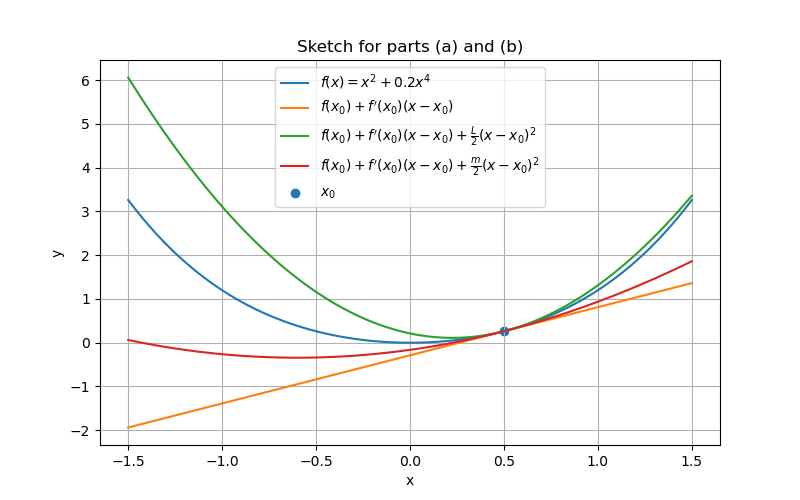
\includegraphics[width=0.9\textwidth]{Figure_1.png}
        \caption{Upper bound (a) and lower bound (b) on $f(y)$.}
    \end{figure}
    \item[(d)] Let $y = x + t v$, $t\in \mathbb{R}$, then
    $$
    \left\{
    \begin{aligned}
    &f(x + t v) \le f(x) + \nabla f(x)^T (t v) + \frac{L}{2}\|t v\|_2^2 = f(x) + t \nabla f(x)^T v + \frac{L}{2} t^2 \|v\|_2^2\\
    &f(x + t v) \ge f(x) + \nabla f(x)^T (t v) + \frac{m}{2}\|t v\|_2^2 = f(x) + t \nabla f(x)^T v + \frac{m}{2} t^2 \|v\|_2^2
    \end{aligned}
    \right.
    $$
    $$
    \Longrightarrow
    \left\{
    \begin{aligned}
    &\frac{f(x + t v) - f(x) - t \nabla f(x)^T v}{\frac{1}{2} t^2 \|v\|_2^2} \le L\\
    &\frac{f(x + t v) - f(x) - t \nabla f(x)^T v}{\frac{1}{2} t^2 \|v\|_2^2} \ge m
    \end{aligned}
    \right.
    $$
    $$
    \xLongrightarrow{t \to 0}
    \left\{
    \begin{aligned}
    &\lim_{t \to 0} \frac{f(x + t v) - f(x) - t \nabla f(x)^T v}{\frac{1}{2} t^2 \|v\|_2^2} = \frac{v^T \nabla^2 f(x) v}{\|v\|_2^2} \le L\\
    &\lim_{t \to 0} \frac{f(x + t v) - f(x) - t \nabla f(x)^T v}{\frac{1}{2} t^2 \|v\|_2^2} = \frac{v^T \nabla^2 f(x) v}{\|v\|_2^2} \ge m
    \end{aligned}
    \right.
    $$
    $$
    \Longrightarrow
    \left\{
    \begin{aligned}
    &\frac{v^T \nabla^2 f(x) v}{\|v\|_2^2} \le L\\
    &\frac{v^T \nabla^2 f(x) v}{\|v\|_2^2} \ge m
    \end{aligned}
    \right.
    \Longleftrightarrow
    \left\{
    \begin{aligned}
    &\nabla^2 f(x) \preceq L I\\
    &\nabla^2 f(x) \succeq m I
    \end{aligned}
    \right.
    \Longrightarrow
    m \leq \lambda(\nabla^2 f(x)) \leq L.
    $$
\end{enumerate}
\end{solution}

\newpage
\begin{exercise}[ ]
	Let $C_1, C_2 \subset \mathbb{R}^n$ be non-empty disjoint closed convex sets, and further assume $C_2$ is bounded.

\begin{enumerate}
    \item[(a)] Show that there exists a hyperplane that strictly separates the two sets.
    \item[(b)] Show that the boundedness assumption is necessary, by giving an example of two closed convex sets that are disjoint but cannot be strictly separated.
\end{enumerate}
\end{exercise}

\newpage

\begin{solution}\textbf{:}
\begin{enumerate}
    \item[(a)] (The following proof comes from my ``Functional Analysis'' course.)
    $$
    \left.
    \begin{aligned}
        &C_2 \text{ is bounded}\\
        &C_2 \text{ is closed}\\
        &C_2 \in \mathbb{R}^n
    \end{aligned}
    \right\}
    \Longrightarrow
    C_2 \text{ is compact.}
    $$
    $$
    \left.
    \begin{aligned}
        &C_1 \text{ is closed}\\
        &C_2 \text{ is compact}\\
        &C_1 \cap C_2 = \emptyset
    \end{aligned}
    \right\}
    \Longrightarrow
    \operatorname{dist} (C_1, C_2) >0
    $$
    (Suppose $\operatorname{dist} (C_1, C_2) = 0$ $\Longrightarrow$ $\inf_{x \in C_1, y \in C_2} \|x-y\| = 0$ $\Longrightarrow$ $\exists$ $\{x_k\} \subseteq C_1$ and $\{y_k\} \subseteq C_2$, s.t. $\|x_k - y_k\| \to 0$.
    
    $\exists$ $\{y_{k_j}\}$, s.t. $y_{k_j} \to y \in C_2$ $\Longrightarrow$ $\|x_{k_j} - y\| \leq \|x_{k_j} - y_{k_j}\| + \|y_{k_j} - y\| \to 0$ as $j \to +\infty$ $\xLongrightarrow{C_1 \text{ is closed}}$ $y \in C_1$ $\Longrightarrow$ $y \in C_1 \cap C_2$, contradicts $C_1 \cap C_2 = \emptyset$.)

    Let $\varepsilon = \frac{1}{4} \operatorname{dist} (C_1, C_2) > 0$, $C_{1_\varepsilon} := C_1 + B(0, \varepsilon)$, $C_{2_\varepsilon} := C_2 + B(0, \varepsilon)$. According to \textit{Hyperplane Separating Theorem}, $\exists$ $f \in X^*$ ($X = \mathbb{R}^n$, $X^*$ is the dual space of $X$), $\exists$ $r \in \mathbb{R}$, s.t. $\sup_{x \in C_{1_\varepsilon}} f(x) < r < \inf_{y \in C_{2_\varepsilon}} f(y)$ $\Longrightarrow$ $\forall$ $x \in C_1$, $\forall$ $y \in C_2$, $z \in B(0,1)$, 
    $$
    r \leq f(y+\varepsilon z) = f(y) + \varepsilon f(z) \Longrightarrow f(-z) \leq \frac{f(y) - r}{\varepsilon}
    $$
    $$
    \Longrightarrow
    \|f\|
    =
    \sup_{z \in B(0,1)} f(-z) \leq \frac{f(y) - r}{\varepsilon}
    $$
    $$
    \Longrightarrow
    r \leq f(y) - \varepsilon \|f\|
    \leq
    \inf_{y \in C_2} f(y) - \varepsilon \|f\|
    <
    \inf_{x \in C_2} f(y)
    $$
    Similarly, $\sup_{x \in C_1} f(x) \leq r$ $\Longrightarrow$ $\sup_{x \in C_1} f(x) <r$.

    In conclusion, $\exists$ $f \in X^*$, $\exists$ $r \in \mathbb{R}$, s.t. $\sup_{x \in C_1} f(x) < r < \inf_{y \in C_2} f(y)$, which means there exists a hyperplane that strictly separates the two sets.
    \item[(b)]
    Let $C_1 = \{(x,y) \in \mathbb{R}^2 \mid x \geq 0, y \geq \frac{1}{x+1}\}$, $C_2 = \{(x,0) \in \mathbb{R}^2 \mid x \geq 0\}$. $C_1$ and $C_2$ are closed and convex, but they cannot be strictly separated by a hyperplane because $\operatorname{dist} (C_1, C_2) = \inf_{x \geq 0} \frac{1}{x+1} = 0$.
\end{enumerate}
\end{solution}

\newpage
\begin{exercise}[ ]
For a convex function $f$ and $x \in \operatorname{int}\;\operatorname{dom} f$, define
\[
S_x := \left\{ s \mid f(y) \ge f(x) + s^T (y-x),\ \forall y \right\}.
\]

\begin{enumerate}
    \item[(a)] Show that $S_x$ is non-empty, convex, and compact. \\
    \textit{[Hint: Supporting hyperplane theorem.]}
    
    \item[(b)] Characterize $S_x$ if $f$ is differentiable at $x$.
\end{enumerate}
\end{exercise}

\newpage

\begin{solution}\textbf{:}
\begin{enumerate}
    \item[(a)]
    \begin{enumerate}
        \item[\ding{172}] $f$ is convex $\Longrightarrow$ $\operatorname{epi} f = \{(x,y) \in \mathbb{R}^{n+1} \mid y \ge f(x)\}$ is convex $\Longrightarrow$ According to the supporting hyperplane theorem, $\exists$ $(\alpha, \beta) \neq 0$, s.t. $\forall$ $(y,t) \in \operatorname{epi} f$, $\alpha^T (y-x) + \beta (t - f(x)) \ge 0$.

        If $\beta < 0$, let $t \to +\infty$, then $\alpha^T (y-x) + \beta (t - f(x)) \to -\infty$, which is a contradiction. Therefore, $\beta \geq 0$.
        
        If $\beta = 0$, then $\alpha \neq 0$ and $\alpha^T (y-x) \ge 0$. $x \in \operatorname{int}\;\operatorname{dom} f$ $\Longrightarrow$ $\exists$ $z \in \operatorname{dom} f$, s.t. $z-x = -a (y-x)$, where $a > 0$. $\alpha^T (z-x) = -a \alpha^T (y-x) \le 0$ $\Longrightarrow$ $\alpha^T (z-x) = 0$, which contradicts $\alpha \neq 0$. Therefore, $\beta \neq 0$.

        In conclusion, $\beta > 0$ $\Longrightarrow$ $\forall$ $y \in \mathbb{R}^n$, $\alpha ^T (y-x) + \beta (f(y) - f(x)) \ge 0$ $\Longrightarrow$ $f(y) \geq f(x) - \frac{\alpha^T}{\beta} (y-x)$ $\Longrightarrow$ $-\frac{\alpha}{\beta} \in S_x$ $\Longrightarrow$ $S_x$ is non-empty.
        \item[\ding{173}] $\forall$ $s_1, s_2 \in S_x$, $\forall$ $\lambda \in [0,1]$, $\forall$ $y \in \mathbb{R}^n$,
        $$
        \left\{
        \begin{aligned}
        &f(y) \ge f(x) + s_1^T (y-x)\\
        &f(y) \ge f(x) + s_2^T (y-x)
        \end{aligned}
        \right.
        \Longrightarrow
        f(y) \ge f(x) + (\lambda s_1 + (1-\lambda) s_2)^T (y-x)
        $$
        $$
        \Longrightarrow
        \lambda s_1 + (1-\lambda) s_2 \in S_x 
        \Longrightarrow 
        S_x \text{ is convex.}
        $$
        \item[\ding{174}] For fixed $y \in \mathbb{R}^n$, $\{s \in \mathbb{R}^n \mid s^T (y-x) \le f(y) - f(x)\}$ is a closed halfspace $\Longrightarrow$
        $$
        S_x = \bigcap_{y \in \mathbb{R}^n} \{s \in \mathbb{R}^n \mid s^T (y-x) \le f(y) - f(x)\}
        $$
        is the intersection of closed halfspaces $\Longrightarrow$ $S_x$ is closed.
        \item[\ding{175}] $x \in \operatorname{int}\;\operatorname{dom} f$ $\Longrightarrow$ $\exists$ $r > 0$, s.t. $B(x,r) \subseteq \operatorname{dom} f$. convex functions are continuous on the interior of their domain $\Longrightarrow$ $\exists$ $M :=\max_{\|z-x\| \leq r} f(z) < +\infty$.
        
        $\forall$ $s \in S_x$, $\forall$ $\|u\| = 1$,
        $$
        \left\{
        \begin{aligned}
        &f(x + r u) \ge f(x) + s^T (r u)\\
        &f(x - r u) \ge f(x) + s^T (-r u)
        \end{aligned}
        \right.
        \Longrightarrow
        |s^T u| \le \frac{M - f(x)}{r} < +\infty
        $$
        Therefore, $S_x$ is bounded.
        \item[\ding{176}] According to \ding{174} and \ding{175},
        $$
        \left\{
        \begin{aligned}
        &S_x \text{ is closed}\\
        &S_x \text{ is bounded}
        \end{aligned}
        \right.
        \Longrightarrow
        S_x \text{ is compact.}
        $$
    \end{enumerate}
    \item[(b)]
    \begin{enumerate}
        \item[\ding{172}] According to the first-order approximation of $f$ at $x$, $f(y) \geq f(x) + \nabla f(x)^T (y-x)$, $\forall$ $y \in \mathbb{R}^n$ $\Longrightarrow$ $\nabla f(x) \in S_x$.
        \item[\ding{173}] Proof by contradiction. Suppose $\exists$ $s \in S_x$, s.t. $s \neq \nabla f(x)$.
        
        Let $y = x + td$, $t > 0$, $\forall$ $d \in \mathbb{R}^n$.
        $$
        f(x+td) \geq f(x) + s^T (td) \Longrightarrow \frac{f(x+td) - f(x)}{t} \geq s^T d
        $$
        Let $t \to 0$, then $\nabla f(x)^T d = \lim_{t \to 0} \frac{f(x+td) - f(x)}{t} \geq s^T d$ $\Longrightarrow$ $(\nabla f(x) - s)^T d \geq 0$, $\forall$ $d \in \mathbb{R}^n$. Let $d = s - \nabla f(x)$, then $(\nabla f(x) - s)^T (s - \nabla f(x)) \geq 0$ $\Longrightarrow$ $\|s - \nabla f(x)\|_2^2 \leq 0$ $\Longrightarrow$ $s = \nabla f(x)$, which is a contradiction. Therefore, $S_x = \{\nabla f(x)\}$.
    \end{enumerate}
\end{enumerate}
\end{solution}

%%%%%%%%%%%%%%%%%%%%%%%%%%%%%%%%%%%%%%%%%%%%%%%%%%%%%%%%%
	
	\newpage
	\newpage
    \bibliography{refs}
    \bibliographystyle{abbrv}
	
\end{document}
